\documentclass[11pt, a4paper]{article}

\usepackage[margin=1in]{geometry}
\usepackage{graphicx}
\usepackage{amsmath, amssymb}
\usepackage{listings}
\usepackage{xcolor}
\usepackage{hyperref}
\usepackage{booktabs}
\usepackage{subcaption}
\usepackage{float}
\usepackage{fancyhdr}
\usepackage{enumitem}

\pagestyle{fancy}
\fancyhf{}
\fancyfoot[C]{\thepage}

\begin{document}

\fancypagestyle{no_hdr_border_rule}{
  \renewcommand{\headrulewidth}{0pt}
}
\thispagestyle{no_hdr_border_rule}

\begin{center}
    {\Large \textbf{Lab 3 -- Report}} \\[0.2cm]
    {\large \textbf{Digital Systems and Microcontrollers (DSM)}} \\[0.1cm]
    {\normalsize International Institute of Information Technology, Hyderabad} \\[0.3cm]
\end{center}

\vspace{0.2cm}
\hrule
\vspace{0.4cm}

\noindent \textbf{Student Name 1:} Manbir Singh Judge \hfill \textbf{Roll Number:} 2026113005 \\
\noindent \textbf{Student Name 2:} Charishma Kandregula \hfill \textbf{Roll Number:} 2026112022 \\
\noindent \textbf{Table Number:} 16 \hfill \textbf{Lab Room Number:} N114 \\
\noindent \textbf{Date of Experiment:} 19/09/2026

\vspace{0.4cm}

\vspace{0.5cm}

\vspace{1em}

\tableofcontents
\vspace{0.5cm}
\hrule
\vspace{0.8cm}

\fancyhead[L]{Lab 3 -- Report}

% ==============================================================================
% experiment 1
% ==============================================================================

\newpage

\fancyhead[R]{Experiment 1}
\section{Experiment 1 -- Binary Half Adder}

\subsection{Aim}
To design, assemble and test binary half adder. 

\subsection{Components \& Equipment Required}

\begin{itemize}
    \item Digital Test Kit (DTK) -- including power supply, switches, indicator LED pairs and breadboard
    \item \textbf{ICs:} 7486-XOR and 7408-AND
    \item Connecting Wires
\end{itemize}

\subsection{Procedure}

\begin{itemize}
    \item Write down Boolean expressions for half adder:
    \begin{itemize}[label=$\circ$]
        \item $S = A \oplus B$
        \item $C = A \cdot B$
    \end{itemize}
    \item Mount the ICs 7486-XOR and 7408-AND. For both ICs, connect $V_{CC}$ to the power rail and $\text{GND}$ to the ground rail.
    \item Setup the circuit according to the Boolean expressions.
    \item Apply inputs to $A$ and $B$ using switches present on the DKT. Connect $S$ and $C$ to LED indicator pairs on the DKT.
    \item Observe and tabulate the outputs for all combinations of inputs and verify the results.
\end{itemize}

\subsection{Observations}

\begin{table}[H]
    \centering
    \caption{Observation for Binary Half Adder}
    \begin{tabular}{|cc|cc|}
        \hline
        $A$ & $B$ & $C$ & $S$ \\
        \hline
        0 & 0 & 0 & 0 \\
        \hline
        0 & 1 & 0 & 1 \\
        \hline
        1 & 0 & 0 & 1 \\
        \hline
        1 & 1 & 1 & 0 \\
        \hline
    \end{tabular}
\end{table}

\subsection{Tinkercad Simulation}
\noindent \textbf{Tinkercad Link:} \href{https://www.tinkercad.com/things/ebDpvZMaMAT-dsm-experiment-3-part-1-and-2?sharecode=TZqAZ21bHZGV4a5mIKK4OJtL0ikV2sPonL3PBrevD4o}{\color{blue}Click here}
\begin{figure}[H]
\centering
    \centering
    
\includegraphics[width=\textwidth]{tc1.png}
    \caption{Tinkercad Simulation Screenshot}
\end{figure}

\subsection{Hardware Setup Photograph}
\begin{figure}[H]
    \centering
    
\includegraphics[width=0.6\textwidth]{lab1.jpeg}
    \caption{Physical Circuit for Binary Half Adder}
\end{figure}

\subsection{Conclusion}
Binary half adder was designed, assembled and tested.

% ==============================================================================
% experiment 2
% ==============================================================================

\newpage

\fancyhead[R]{Experiment 2}
\section{Experiment 2 -- Binary Full Adder}

\subsection{Aim}
To design, assemble and test binary full adder. 

\subsection{Components \& Equipment Required}

\begin{itemize}
    \item Digital Test Kit (DTK) -- including power supply, switches, indicator LED pairs and breadboard
    \item \textbf{ICs:} 7486-XOR and 7408-AND
    \item Connecting Wires
\end{itemize}

\subsection{Procedure}

\begin{itemize}
    \item Write down Boolean expressions for full adder:
    \begin{itemize}[label=$\circ$]
        \item First half adder sum, $S_1 = A \oplus B$
        \item First half adder carry, $C_1 = A \cdot B$
        \item Second half adder carry, $C_2 = S_1 \cdot C_{in}$
        \item Sum, $S = S_1 \oplus C_{in}$
        \item Final carry, $C_{out} = C_1 + C_2$ \hfill
    \end{itemize}
    \item Modify the Boolean expression to remove the need for a seperate OR gate:
    \begin{itemize}[label=$\circ$]
        \item Notice that, $C_1 =$ implies $A = 1$ and $B = 1$. Which means, $C_2 = (A \oplus B) \cdot C_{in} = (1 \oplus 1) \cdot C_{in} = 0 \cdot C_{in} = 0$.
        \item Hence, both $C_1$ and $C_2$ can't be $1$ simultaneously, i.e., they are mutually exclusive.
        \item For mutually exclusive terms, OR and XOR provide the same result.
        \item Hence, $C_{out} = C_1 + C_2 = C_1 \oplus C_2$
    \end{itemize}
    \item Mount the ICs 7486-XOR and 7408-AND. For both ICs, connect $V_{CC}$ to the power rail and $\text{GND}$ to the ground rail.
    \item Setup the circuit according to the Boolean expressions.
    \item Apply inputs to $A$, $B$ and $C_{in}$ using switches present on the DKT. Connect $S$ and $C_{out}$ to LED indicator pairs on the DKT.
    \item Observe and tabulate the outputs for all combinations of inputs and verify the results.
\end{itemize}

\subsection{Observations}

\begin{table}[H]
    \centering
    \caption{Observation for Binary Full Adder}
    \begin{tabular}{|ccc|cc|}
        \hline
        $A$ & $B$ & $C_{in}$ & $C$ & $S$ \\
        \hline
        0 & 0 & 0 & 0 & 0 \\
        \hline
        0 & 0 & 1 & 0 & 1 \\
        \hline
        0 & 1 & 0 & 0 & 1 \\
        \hline
        0 & 1 & 1 & 1 & 0 \\
        \hline
        1 & 0 & 0 & 0 & 1 \\
        \hline
        1 & 0 & 1 & 1 & 0 \\
        \hline
        1 & 1 & 0 & 1 & 0 \\
        \hline
        1 & 1 & 1 & 1 & 1 \\
        \hline
    \end{tabular}
\end{table}

\subsection{Tinkercad Simulation}
\noindent \textbf{Tinkercad Link:} \href{https://www.tinkercad.com/things/ebDpvZMaMAT-dsm-experiment-3-part-1-and-2?sharecode=TZqAZ21bHZGV4a5mIKK4OJtL0ikV2sPonL3PBrevD4o}{\color{blue}Click here}
\begin{figure}[H]
\centering
    \centering
    
\includegraphics[width=\textwidth]{tc2.png}
    \caption{Tinkercad Simulation Screenshot}
\end{figure}

\subsection{Hardware Setup Photograph}
\begin{figure}[H]
    \centering
    
\includegraphics[width=0.6\textwidth]{lab2.jpeg}
    \caption{Physical Circuit for Binary Full Adder}
\end{figure}

\subsection{Conclusion}
Binary full adder was designed, assembled and tested.

% ==============================================================================
% experiment 3
% ==============================================================================

\newpage

\fancyhead[R]{Experiment 3}
\section{Experiment 3 -- Binary Half Subtractor}

\subsection{Aim}
To design, assemble and test binary half subtractor. 

\subsection{Components \& Equipment Required}

\begin{itemize}
    \item Digital Test Kit (DTK) -- including power supply, switches, indicator LED pairs and breadboard
    \item \textbf{ICs:} 7486-XOR and 7408-AND
    \item Connecting Wires
\end{itemize}

\subsection{Procedure}

\begin{itemize}
    \item Write down Boolean expressions for half subtractor:
    \begin{itemize}[label=$\circ$]
        \item Difference, $D = A \oplus B$
        \item Borrow, $B_{out} = \overline{A} \cdot B$
    \end{itemize}
    \item Modify the Boolean expression to remove the need for a seperate NOT gate:
    \begin{itemize}[label=$\circ$]
        \item We know that, $A \oplus 1 = \overline{A}$.
        \item Therefore, $B_{out} = (A \oplus 1) \cdot B$
    \end{itemize}
    \item Mount the ICs 7486-XOR and 7408-AND. For both ICs, connect $V_{CC}$ to the power rail and $\text{GND}$ to the ground rail.
    \item Setup the circuit according to the Boolean expressions.
    \item Apply inputs to $A$ and $B$ using switches present on the DKT. Connect $D$ and $B_{out}$ to LED indicator pairs on the DKT.
    \item Observe and tabulate the outputs for all combinations of inputs and verify the results.
\end{itemize}

\subsection{Observations}

\begin{table}[H]
    \centering
    \caption{Observation for Binary Half Subtractor}
    \begin{tabular}{|cc|cc|}
        \hline
        $A$ & $B$ & $B_{out}$ & $D$ \\
        \hline
        0 & 0 & 0 & 0 \\
        \hline
        0 & 1 & 1 & 1 \\
        \hline
        1 & 0 & 0 & 1 \\
        \hline
        1 & 1 & 0 & 0 \\
        \hline
    \end{tabular}
\end{table}

\subsection{Tinkercad Simulation}
\noindent \textbf{Tinkercad Link:} \href{https://www.tinkercad.com/things/fnvClRjKQg0-dsm-experiment-3-part-3?sharecode=cYCmQMRLdYlVF9FCfp8gIeCjlj78PSv52U0TRZrD8QU}{\color{blue}Click here}
\begin{figure}[H]
\centering
    \centering
    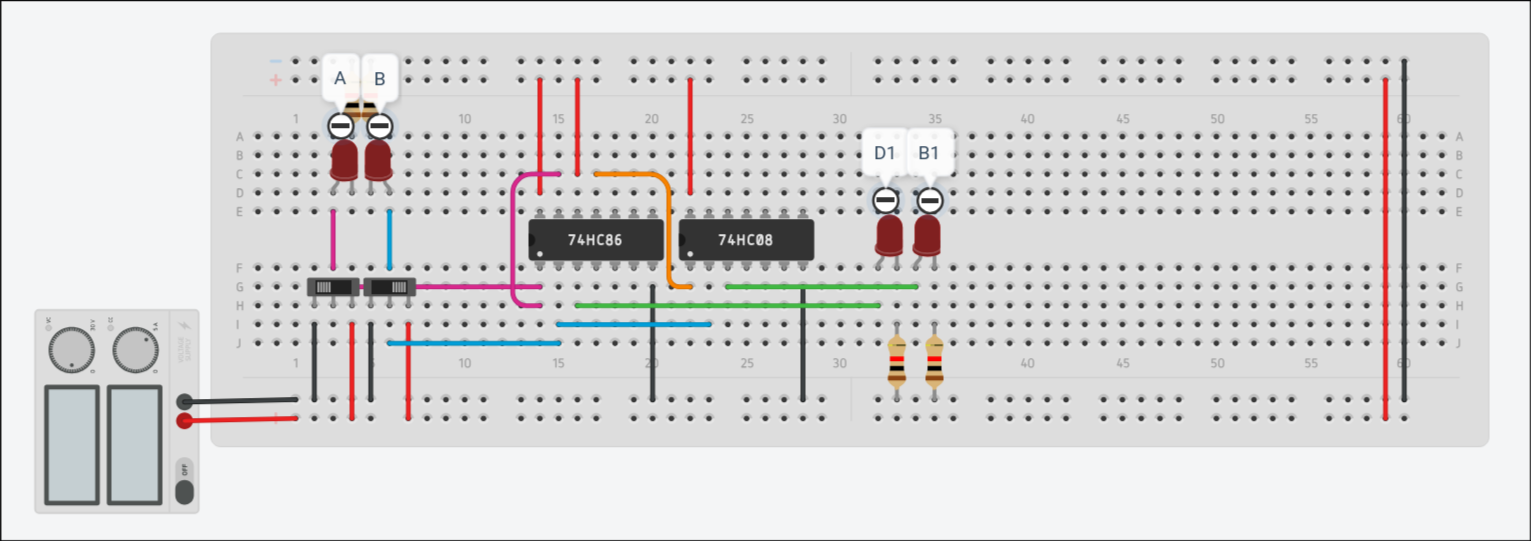
\includegraphics[width=\textwidth]{tc3.png}
    \caption{Tinkercad Simulation Screenshot}
\end{figure}

\subsection{Hardware Setup Photograph}
\begin{figure}[H]
    \centering
    
\includegraphics[width=0.6\textwidth]{lab3.jpeg}
    \caption{Physical Circuit for Binary Half Subtractor}
\end{figure}

\subsection{Conclusion}
Binary half subtractor was designed, assembled and tested.

% ==============================================================================
% experiment 4
% ==============================================================================

\newpage

\fancyhead[R]{Experiment 4}
\section{Experiment 4 -- Binary Full Subtractor}

\subsection{Aim}
To design, assemble and test binary full subtractor. 

\subsection{Components \& Equipment Required}

\begin{itemize}
    \item Digital Test Kit (DTK) -- including power supply, switches, indicator LED pairs and breadboard
    \item \textbf{ICs:} 7486-XOR and 7408-AND
    \item Connecting Wires
\end{itemize}

\subsection{Procedure}

\begin{itemize}
    \item Write down Boolean expressions for half adder:
    \begin{itemize}[label=$\circ$]
        \item First half subtractor difference, $D_1 = A \oplus B$
        \item Difference, $D = D_1 \oplus B_{in}$
        \item First half subtractor borrow, $B_1 = \overline{A} \cdot B$
        \item Second half subtractor borrow, $B_2 = \overline{D_1} \cdot B_{in} = D \cdot B_{in}$
        \item Output borrow, $B_{out} = B_1 + B_2$
    \end{itemize}
    \item Modify the Boolean expression to :
    \begin{itemize}[label=$\circ$]
        \item We already know, $B_1 = (A \oplus 1) \cdot B$
        \item Notice, $B_1$ and $B_2$ are mutually exclusive by writing down they truth table. Hence, $B_{out} = B_1 \oplus B_2$.
        \item Now, $B_2 = \overline{D_1} \cdot B_{in}$
        \begin{itemize}[label={$=$}]
            \item $\overline{D_1} B_{in} + 0$
            \item $\overline{D_1} B_{in} B_{in} + D_1 B_{in} \overline{B_{in}}$
            \item $B_{in} (\overline{D_1} B_{in} + D_1 \overline{B_{in}})$
            \item $B_{in} (D_1 \oplus B_{in})$
            \item $D B_{in}$
        \end{itemize}
    \end{itemize}
    \item Note the final Boolean expressions:
    \begin{itemize}[label=$\circ$]
        \item $D_1 = A \oplus B$
        \item $D = D_1 \oplus B_{in}$
        \item $B_1 = (A \oplus 1) \cdot B$ \hfill [modified]
        \item $B_2 = D \cdot B_{in}$ \hfill [modified]
        \item $B_{out} = B_1 \oplus B_2$ \hfill [modified]
    \end{itemize}
    \item Mount the ICs 7486-XOR and 7408-AND. For both ICs, connect $V_{CC}$ to the power rail and $\text{GND}$ to the ground rail.
    \item Setup the circuit according to the final Boolean expressions.
    \item Apply inputs to $A$, $B$ and $B_{in}$ using switches present on the DKT. Connect $D$ and $B_{out}$ to LED indicator pairs on the DKT.
    \item Observe and tabulate the outputs for all combinations of inputs and verify the results.
\end{itemize}

\subsection{Observations}

\begin{table}[H]
    \centering
    \caption{Observation for Binary Full Subtractor}
    \begin{tabular}{|ccc|cc|}
        \hline
        $A$ & $B$ & $B_{in}$ & $B_{out}$ & $D$ \\
        \hline
        0 & 0 & 0 & 0 & 0 \\
        \hline
        0 & 0 & 1 & 1 & 1 \\
        \hline
        0 & 1 & 0 & 1 & 1 \\
        \hline
        0 & 1 & 1 & 1 & 0 \\
        \hline
        1 & 0 & 0 & 0 & 1 \\
        \hline
        1 & 0 & 1 & 0 & 0 \\
        \hline
        1 & 1 & 0 & 0 & 0 \\
        \hline
        1 & 1 & 1 & 1 & 1 \\
        \hline
    \end{tabular}
\end{table}

\subsection{Tinkercad Simulation}
\noindent \textbf{Tinkercad Link:} \href{https://www.tinkercad.com/things/d1FqF97gTOR-dsm-experiment-3-part-4?sharecode=CcVcad4-vT3XXqIVOh77uDOH8632an0Vxnek2zZFvnY}{\color{blue}Click here}
\begin{figure}[H]
\centering
    \centering
    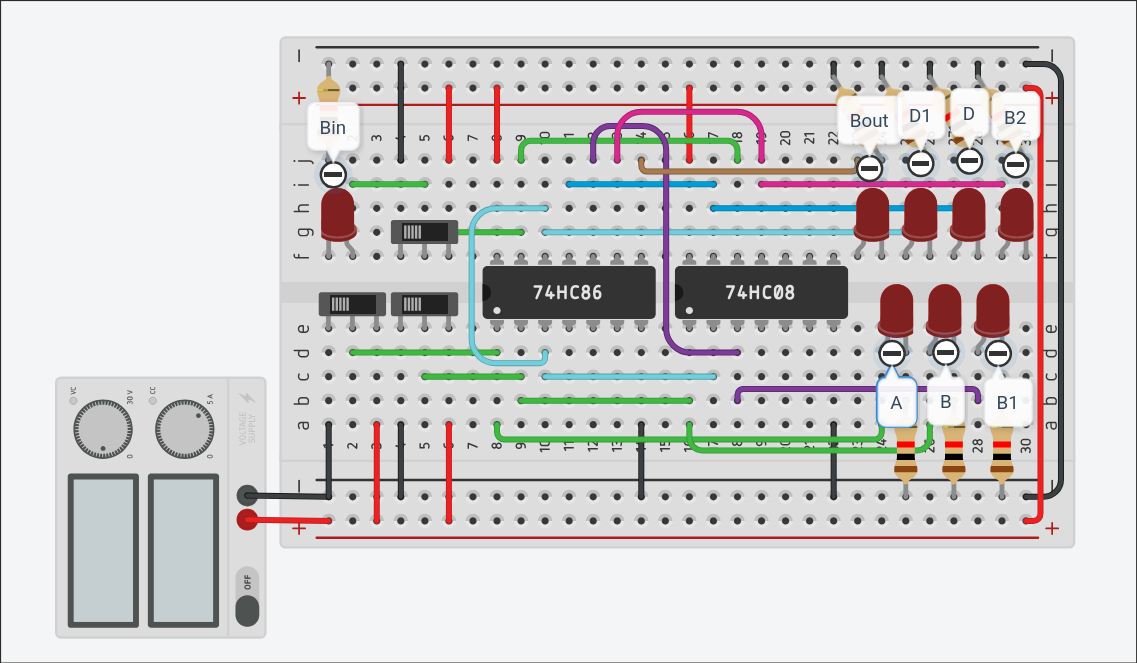
\includegraphics[width=0.75\textwidth]{tc4.png}
    \caption{Tinkercad Simulation Screenshot}
\end{figure}

\subsection{Hardware Setup Photograph}
\begin{figure}[H]
    \centering
    
\includegraphics[width=0.6\textwidth]{lab4.jpeg}
    \caption{Physical Circuit for Binary Full Subtractor}
\end{figure}

\subsection{Conclusion}
Binary full subtractor was designed, assembled and tested.

\end{document}